\documentclass{article}
\usepackage{graphicx}

\begin{document}

\title{Report}

\section{Plots}
\subsection{Final Performance}
\begin{figure}[h]
    \centering
    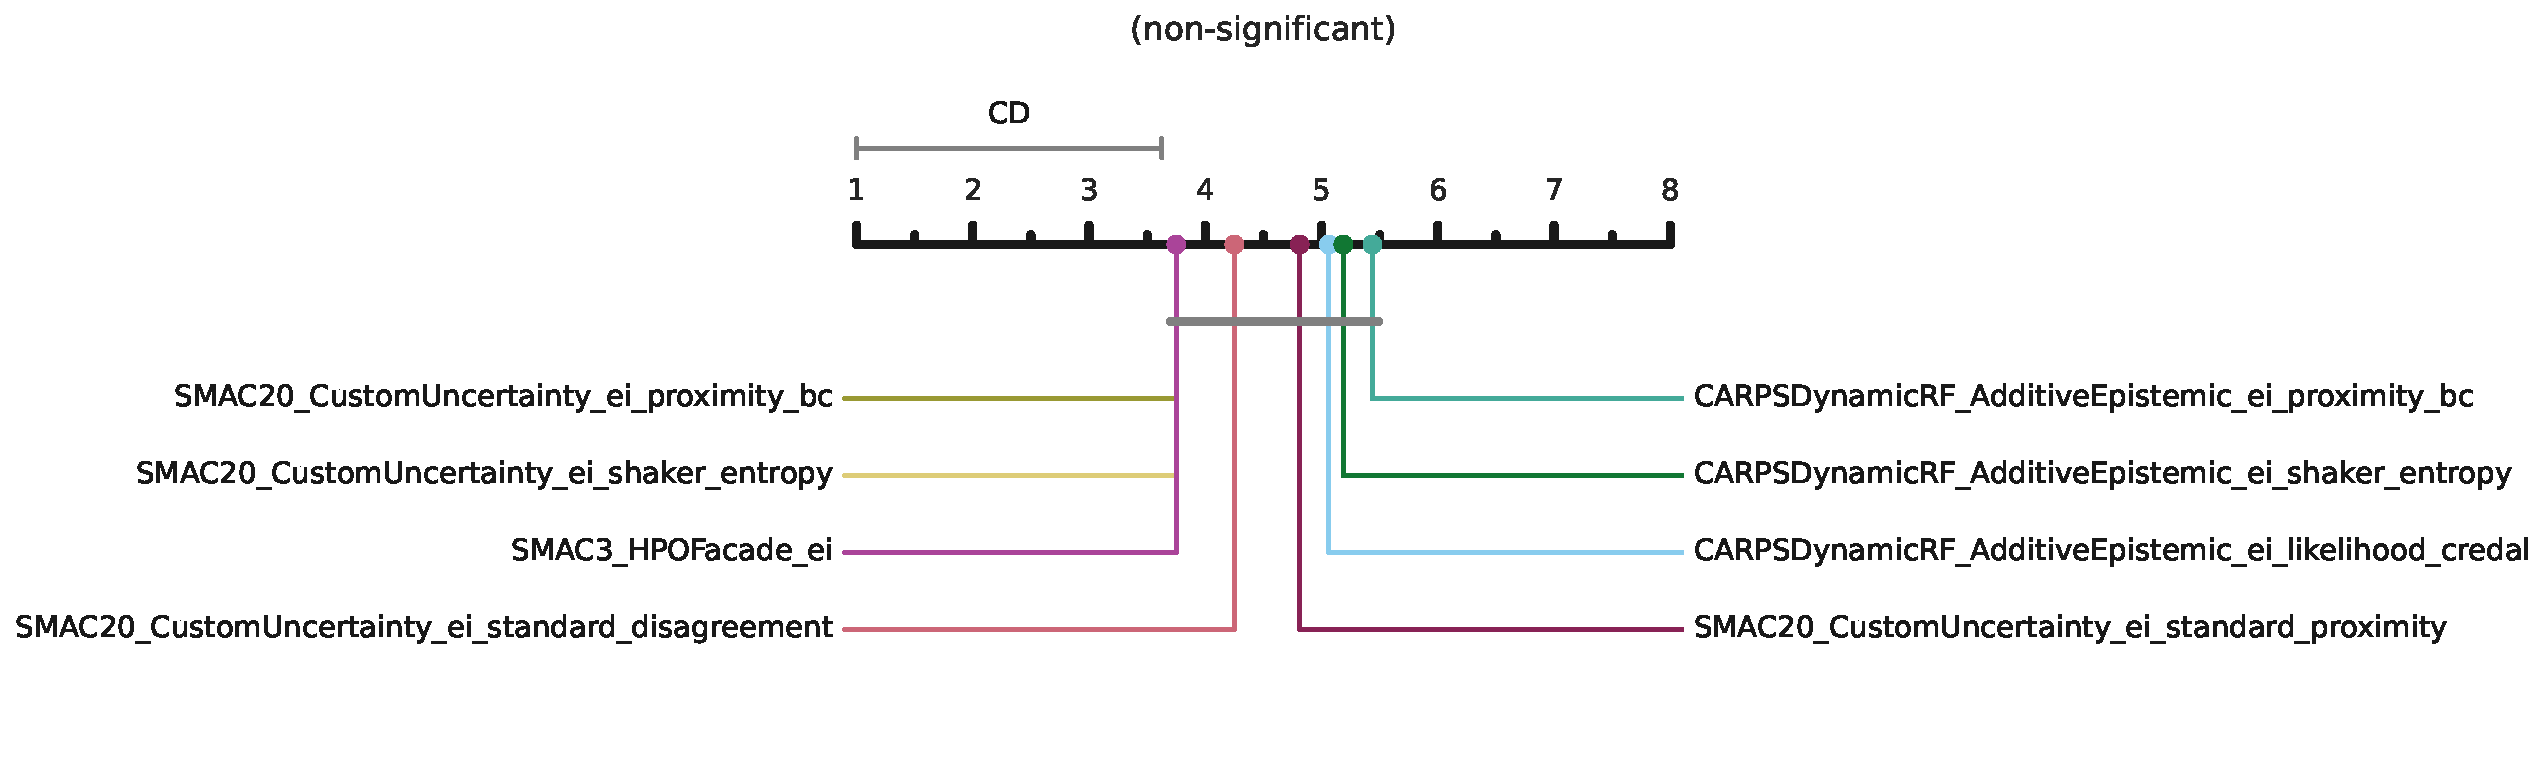
\includegraphics[width=0.9\textwidth]{figures/blackbox_test_criticaldifference}
    \caption{Task Type: blackbox - Set: test - Critical Difference}
    \label{fig:figures/blackbox_test_criticaldifference}
\end{figure}

\begin{figure}[h]
    \centering
    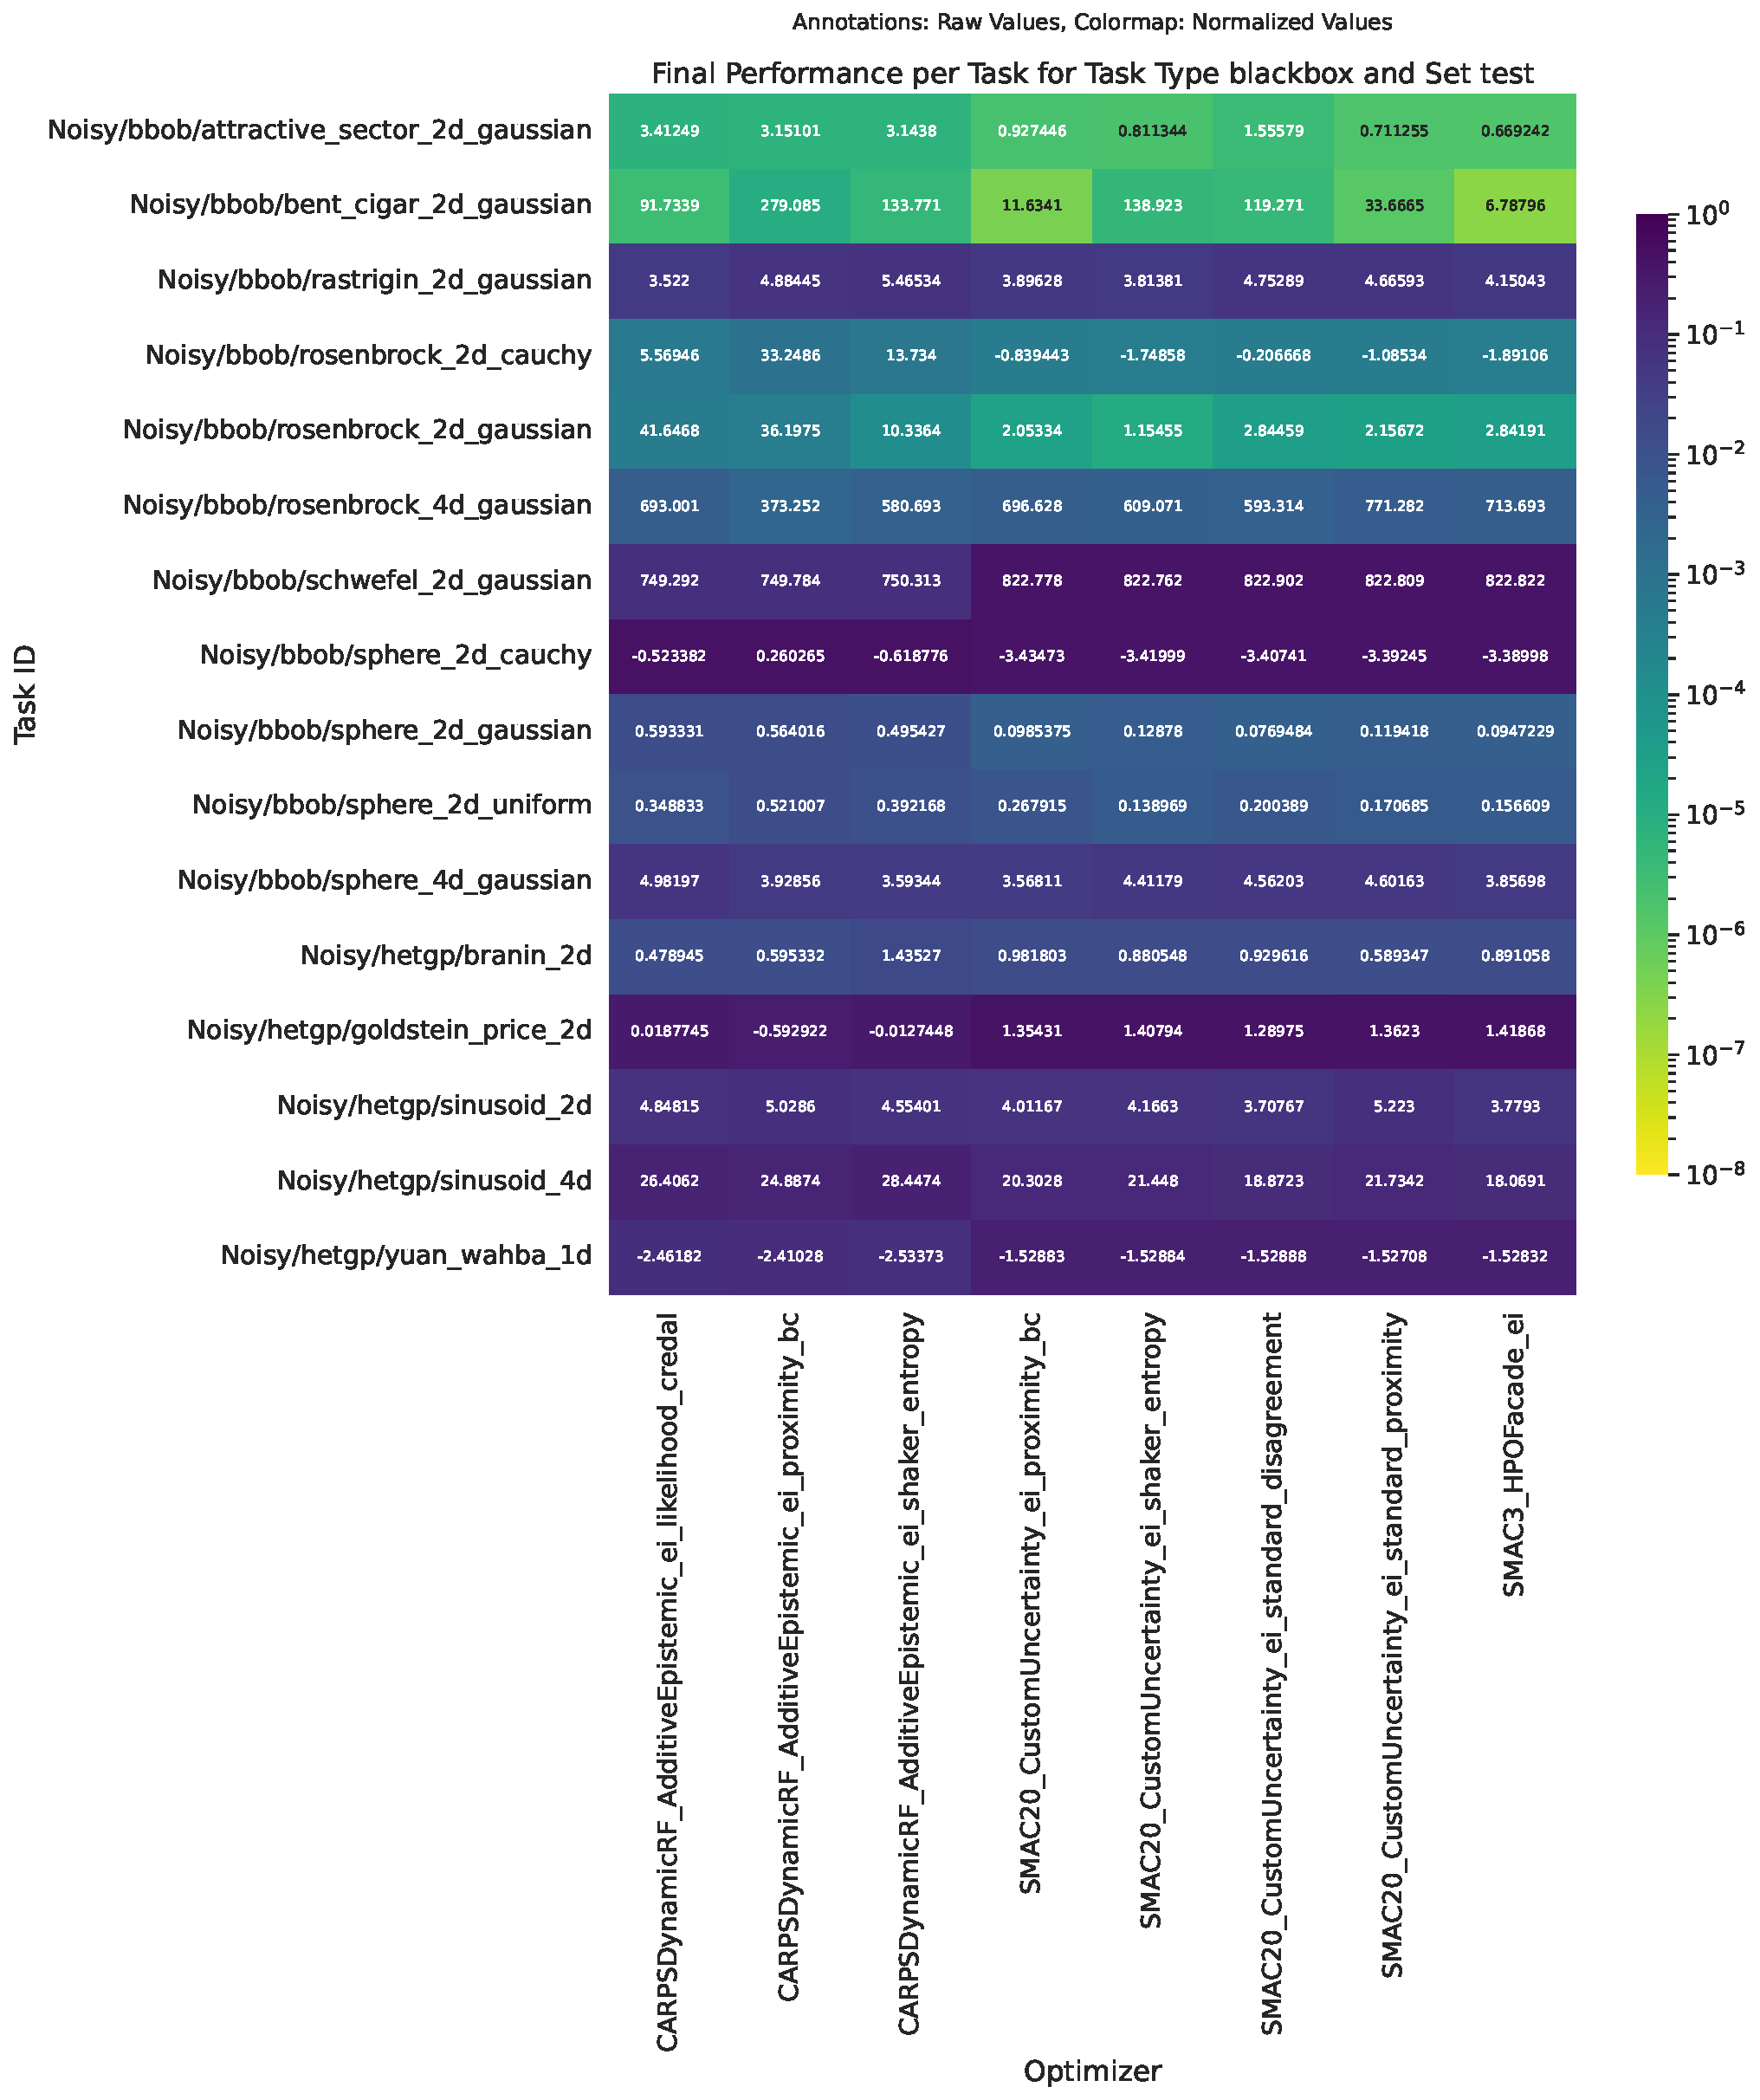
\includegraphics[width=0.9\textwidth]{figures/blackbox_test_performancepertask}
    \caption{Task Type: blackbox - Set: test - Performance per Task}
    \label{fig:figures/blackbox_test_performancepertask}
\end{figure}

\subsection{Anytime Performance}
\begin{figure}[h]
    \centering
    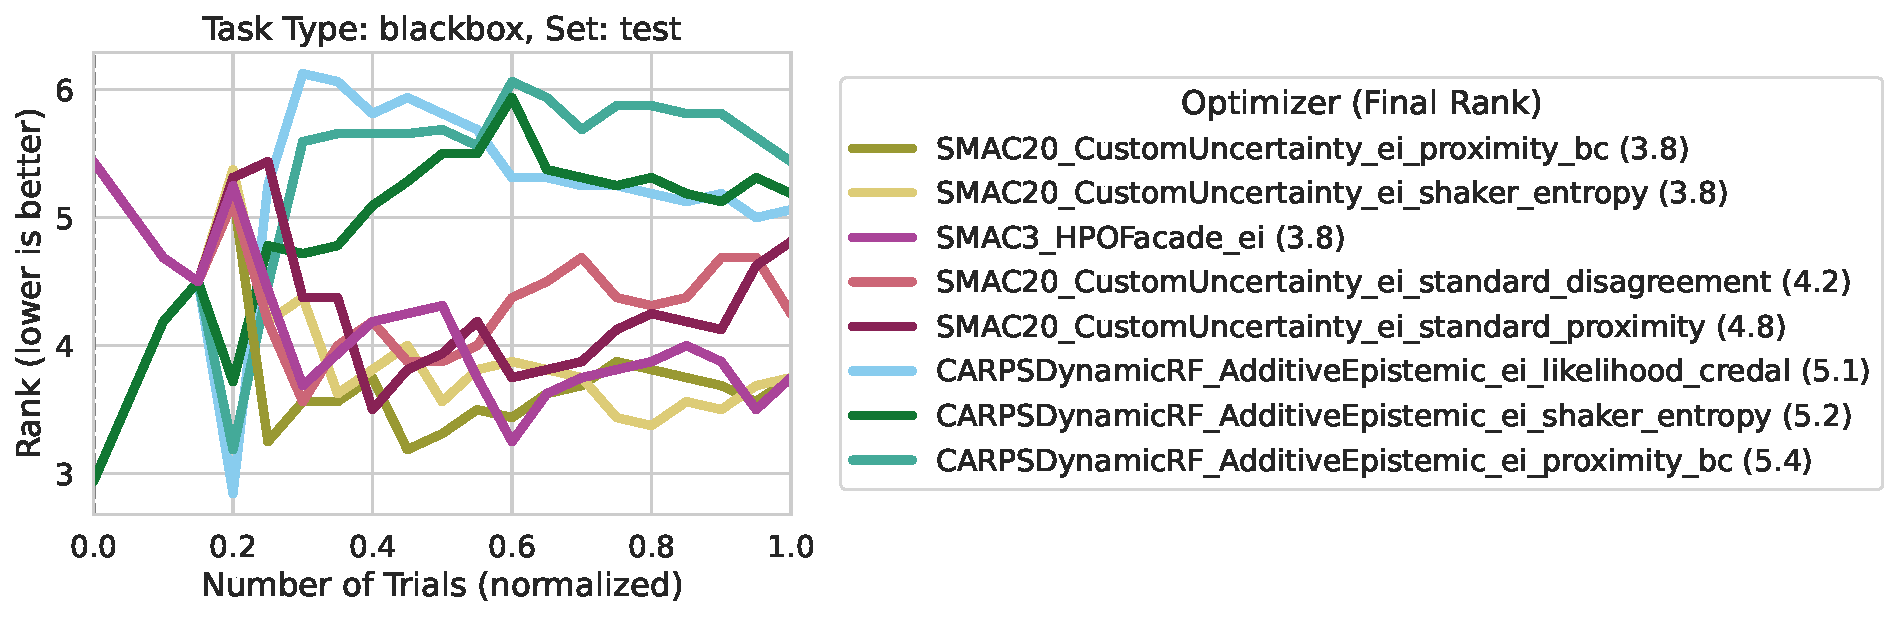
\includegraphics[width=0.9\textwidth]{figures/blackbox_test_rank}
    \caption{Task Type: blackbox - Set: test - Rank over Time}
    \label{fig:figures/blackbox_test_rank}
\end{figure}

\section{Explanation of Plots}
\subsection{Final Performance}
\subsubsection{Critical Difference}
Most importantly, we propose statistical testing on rankings as our main result. For the ranking, we use the library \code{autorank}~\citep{herbold-joss20} for determining the ranks and critical differences. The ranking is performed on the raw performance values, averaged across seeds. To be more precise, we use the frequentist approach~\citep{demsar-06a}: We use the non-parametric Friedman test as an omnibus test to determine whether there are any significant differences between the median values of the populations. We use this test because we have more than two populations, which cannot be assumed to be normally distributed. We use the post hoc Nemenyi test to infer which differences are significant. The significance level is $lpha=0.05$. In order to be considered different, the difference between the mean ranks of two optimizers must be greater than the critical difference (CD).

\subsubsection{Performance per Task}
The heatmap shows the performance of the optimizers per task. The performance is first log-transformed, then normalized and averaged over seeds. The performance is shown as a heatmap, where the colors indicate the performance of the optimizer on a specific task. The better the optimizer performs, the lighter/more yellow the color.

\subsection{Anytime Performance}
\subsubsection{Rank over Time}
The rank of each optimizer over time compares which optimizer performs better, the lower the rank the better. For each optimizer and task, the performance is averaged over seeds to obtain an estimate of the performance. The rank is then calculated per step and task with the same approach as for the critical difference diagram. The grey area marks the area where the test results are insignificant.



\end{document}
